\chapter{Mesh and Tours Networks}

The \textit{mesh} and the \textit{torus} networks have processing units disposed as a grid. In a sense, they are the two dimensional versions of the linear array and ring, respectively. There are actually even more general mesh and torus architectures, defined for any number of dimensions, but we will focus on the basic 2-D versions.

A mesh (or torus) with $P$ processing units can be drawn as a grid of side $\sqrt{P}$. In the mesh each inner processor has 4 links, to the four cardinal directions, while processors along the edges have fewer links, either 3 or 2 depending on their position. On the other hand, in the torus, similarly to the ring, all processors have 4 links, those along the edges simply have connections looping back to the opposite edge of the network. In this kind of network, it is often useful to use two indices, instead of just one, to identify processors, the first for the "row" and the second for the "column" of the network, as done for the elements of a matrix. Such indices will then range over the set $\{0, 1, \ldots, \sqrt{P}-1\}$. Also in this case, we will assume that each processing unit knows its pair of indices.

\vspace{-4em}

\begin{figure}[H]
    \centering
    % \hspace{2cm}
    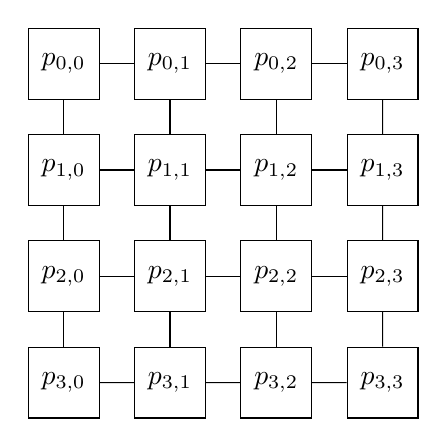
\begin{tikzpicture}[scale=0.9, every node/.style={scale=1}, baseline=(p30.base)]
        % Draw the grid of nodes
        \foreach \i in {0,1,2,3} {
            \foreach \j in {0,1,2,3} {
                \node[draw, minimum size=0.9cm] (p\i\j) at (1.5*\j, -1.5*\i) {$p_{\i,\j}$};
            }
        }
        % Draw the horizontal connections
        \foreach \i in {0,1,2,3} {
            \foreach \j in {0,1,2} {
                \draw (p\i\j) -- (p\i\the\numexpr\j+1\relax);
            }
        }
        % Draw the vertical connections
        \foreach \i in {0,1,2} {
            \foreach \j in {0,1,2,3} {
                \draw (p\i\j) -- (p\the\numexpr\i+1\relax\j);
            }
        }
    \end{tikzpicture}
    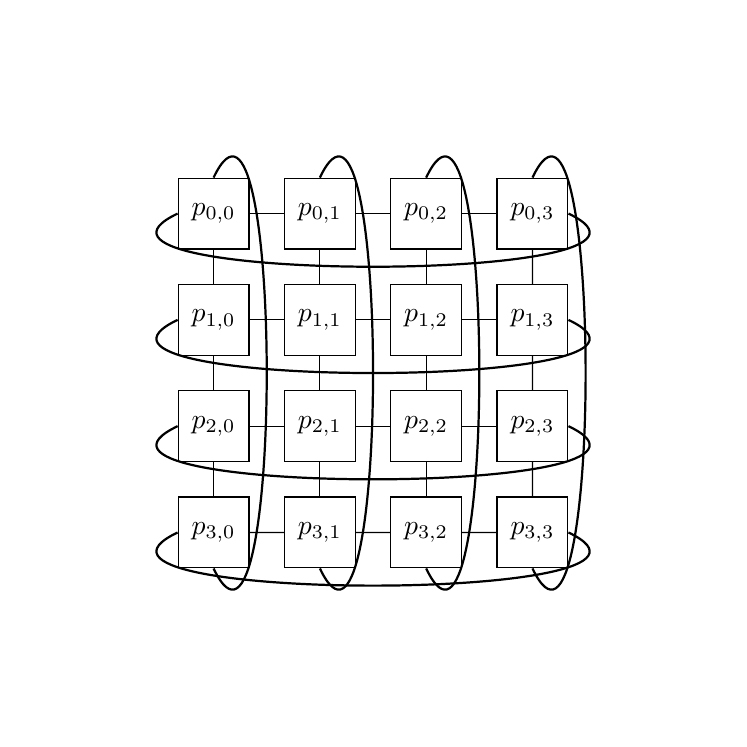
\begin{tikzpicture}[scale=0.9, every node/.style={scale=1}, baseline=(p30.base)]
        % Draw the grid of nodes
        \foreach \i in {0,1,2,3} {
            \foreach \j in {0,1,2,3} {
                \node[draw, minimum size=0.9cm] (p\i\j) at (1.5*\j, -1.5*\i) {$p_{\i,\j}$};
            }
        }
        % Draw the horizontal connections
        \foreach \i in {0,1,2,3} {
            \foreach \j in {0,1,2} {
                \draw (p\i\j) -- (p\i\the\numexpr\j+1\relax);
            }
        }
        % Draw the vertical connections
        \foreach \i in {0,1,2} {
            \foreach \j in {0,1,2,3} {
                \draw (p\i\j) -- (p\the\numexpr\i+1\relax\j);
            }
        }
        % Define offsets for curve controls (tune these for appearance)
        \def\hCtrlOut{2.1}  % How far "out" horizontally the control point is from the node anchor
        \def\hCtrlBend{1} % How much "bend" (vertical offset) for horizontal wraps
        \def\vCtrlOut{2.1}   % How far "out" vertically the control point is from the node anchor
        \def\vCtrlBend{1}  % How much "bend" (horizontal offset) for vertical wraps

        % Draw the wrap-around horizontal connections (torus)
        \foreach \i in {0,1,2,3} {
            % Determine vertical direction of the arc based on row index
            \pgfmathsetmacro{\currentVBend}{-\hCtrlBend}
            \draw [thick] (p\i0.west) .. controls +(-\hCtrlOut, \currentVBend) and +(\hCtrlOut, \currentVBend) .. (p\i3.east);
        }
        
        % Draw the wrap-around vertical connections (torus)
        \foreach \j in {0,1,2,3} {
            % Determine horizontal direction of the arc based on column index
            \pgfmathsetmacro{\currentHBend}{\vCtrlBend}
            \draw [thick] (p0\j.north) .. controls +(\currentHBend, \vCtrlOut) and +(\currentHBend, -\vCtrlOut) .. (p3\j.south);
        }
    \end{tikzpicture}
    \hspace{-2cm}

    \vspace{-3em}

    \caption{$4 \times 4$ mesh (left) and torus with 16 processing units (right)}
    \label{fig:torus}
\end{figure}

\subsubsection{Properties of the Mesh and Torus}


A \textbf{mesh} $M_P$ with $P$ processors and bidirectional links has:
\begin{itemize}
    \item \textbf{Diameter} $\mathit{diam}(M_P) = 2\sqrt{P} - 2$, i.e. the distance between two opposite corners.
    \item \textbf{Bisection bandwidth} $b(M_P) = \sqrt{P} + (\sqrt{P} \bmod 2)$.
\end{itemize}

A \textbf{torus} $T_P$ with $P$ processors and bidirectional links has:
\begin{itemize}
    \item \textbf{Diameter} $\mathit{diam}(T_P) = 2\lfloor \sqrt{P}/2 \rfloor$, i.e. the distance between any two opposite (horizontally and vertically) processors.
    \item \textbf{Bisection bandwidth} $b(T_P) = 2\sqrt{P} + 2(\sqrt{P} \bmod 2)$.
\end{itemize}


\section{Transitive Closure of a Graph}

The \textbf{transitive closure} of a (directed) graph $G = (V, E)$ is denoted by $G^* = (V, E^*)$, where $E^* = \{(u, v) \in V \times V \mid$ there is a (directed) path from $u$ to $v\}$. This fundamental operation is particularly useful when a graph represents relationships between objects, such as dependencies, reachability, or hierarchical structures.

Without loss of generality, we can represent the nodes of $V$ as consecutive integers, i.e., $V = \{0, 1, \ldots, |V| - 1\}$. The adjacency matrix $A$ of $G$ is an $|V| \times |V|$ matrix where each element $A_{i,j}$ for $i, j \in V$ is defined as:
$$
    A_{i,j} = \begin{cases}
        1 & \text{if } (i, j) \in E \\
        0 & \text{otherwise}
    \end{cases}
$$
The transitive closure $A^*$ of the adjacency matrix $A$, is simply the adjacency matrix of $G^*$.

Before diving into the parallel algorithm, let's outline the general procedure for computing the transitive closure. The algorithm proceeds through $|V|$ distinct phases, with each phase potentially augmenting the graph with new edges based on the current state. We represent the graph at the start of phase $k$ as $G^k = (V, E^k)$ and at the end as $G^{k+1} = (V, E^{k+1})$. Starting with the original graph $G^0 = G$, the algorithm transforms it through all phases until reaching $G^{|V|}$, which we will prove is equivalent to the transitive closure $G^*$.

During each phase $0 \leq k < |V|$, we update the graph according to the rule:
$E^{k+1} = E^k \cup \{(i, j) \in V \times V \mid (i, k), (k, j) \in E^k\}$.
In simpler terms, if phase $k$ finds edges from $i$ to $k$ and from $k$ to $j$ in $G^k$, it adds a new edge from $i$ to $j$ in $G^{k+1}$.

The key to proving that $G^{|V|}$ is indeed the transitive closure lies in this observation: for any $0 \leq k \leq |V|$, an edge $(i, j)$ exists in $G^k$ if and only if the original graph $G$ contains a path from $i$ to $j$ that passes only through nodes in $\{0, 1, \ldots, k-1\}$ (excluding $i$ and $j$ themselves). When we reach phase $|V| - 1$, this set encompasses all nodes in $V$, making $G^{|V|}$ the complete transitive closure.

We can prove this observation through induction on $k$. For the base case $k = 0$, $G^0 = G$ contains only the original edges, which represent paths without intermediate nodes (since $\{0, \ldots, k-1\} = \emptyset$). For the inductive step, assume the property holds for some $k \geq 0$. In phase $k$, we add edges $(i, j)$ whenever $G^k$ contains edges $(i, k)$ and $(k, j)$. By our inductive hypothesis, this means $G$ has paths from $i$ to $k$ and from $k$ to $j$ that only use nodes in $\{0, \ldots, k-1\}$. Combining these paths creates a path from $i$ to $j$ that uses nodes in $\{0, \ldots, k\}$, thus proving the property for $k + 1$.

\vspace{-1em}

\begin{figure}[H]
\centering
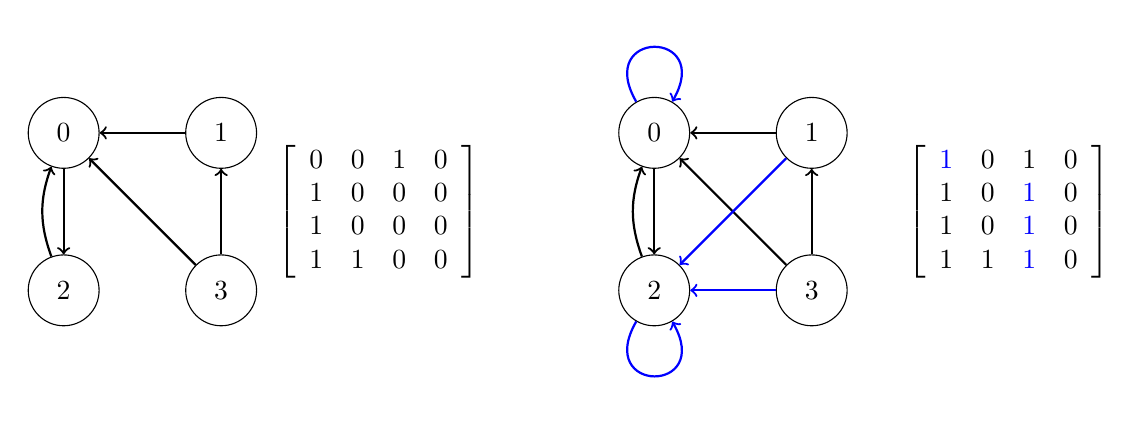
\begin{tikzpicture}[scale=1, every node/.style={scale=1}]
    % Left: Original graph
    \begin{scope}
        % Nodes
        \node[circle,draw,minimum size=0.9cm] (a) at (0,2) {0};
        \node[circle,draw,minimum size=0.9cm] (b) at (2,2) {1};
        \node[circle,draw,minimum size=0.9cm] (c) at (0,0) {2};
        \node[circle,draw,minimum size=0.9cm] (d) at (2,0) {3};
        % Edges
        \draw[->,thick] (b) -- (a);
        \draw[->,thick] (a) -- (c);
        \draw[->,thick] (c) to [bend left=20] (a);
        \draw[->,thick] (d) -- (a);
        \draw[->,thick] (d) -- (b);
    \end{scope}
    % Left: Adjacency matrix
    \node at (4,1) {$\left[\begin{array}{cccc}
        0 & 0 & 1 & 0 \\
        1 & 0 & 0 & 0 \\
        1 & 0 & 0 & 0 \\
        1 & 1 & 0 & 0
    \end{array}\right]$};

    % Right: Transitive closure
    \begin{scope}[xshift=7.5cm]
        % Nodes
        \node[circle,draw,minimum size=0.9cm] (a) at (0,2) {0};
        \node[circle,draw,minimum size=0.9cm] (b) at (2,2) {1};
        \node[circle,draw,minimum size=0.9cm] (c) at (0,0) {2};
        \node[circle,draw,minimum size=0.9cm] (d) at (2,0) {3};
        % Original edges
        \draw[->,thick] (b) -- (a);
        \draw[->,thick] (c) to [bend left=20] (a);
        \draw[->,thick] (a) -- (c);
        \draw[->,thick, blue] (d) -- (c);
        \draw[->,thick] (d) -- (b);
        % New edges in blue
        \draw[->,thick,blue] (a) to [out=120,in=60,looseness=6] (a); % self-loop 0
        \draw[->,thick,blue] (c) to [out=240,in=300,looseness=6] (c); % self-loop 2
        \draw[->,thick] (d) -- (a);
        \draw[->,thick,blue] (b) -- (c);
    \end{scope}
    % Right: Transitive closure adjacency matrix
    \node at (12,1) {$\left[\begin{array}{cccc}
        \textcolor{blue}{1} & 0 & 1 & 0 \\
        1 & 0 & \textcolor{blue}{1} & 0 \\
        1 & 0 & \textcolor{blue}{1} & 0 \\
        1 & 1 & \textcolor{blue}{1} & 0
    \end{array}\right]$};
\end{tikzpicture}

\caption{A graph and its adjacency matrix (left) and their transitive closures (right). The edges in blue are the new ones added in the transitive closure.}
\label{fig:transitive-closure}
\end{figure}

\vspace{-1em}

We can now explain the parallel algorithm to compute the transitive closure of a directed graph $G = (V, E)$ with $|V| = N$ nodes, on a mesh with the same size of the corresponding adjacency matrix $A$, that is, with $P = N^2$ processing units with constant memory.

The algorithm implements the $N$ phases described above in a systolic fashion. Unlike previous systolic algorithms, each phase requires multiple steps, though some steps from different phases can be executed in parallel. The algorithm operates directly on the adjacency matrix $A$, which enters the mesh one row at a time from the top, with each element being assigned to its corresponding processing unit in the first row.

A key difference from the systolic algorithms we saw for linear array networks is that data doesn't automatically advance to the next row at each step. Instead, when a row $A_i$ enters the mesh, it stops at the first available row. Since the matrix is input starting with row $A_0$, which stops at row 0, followed by subsequent rows, each row $A_i$ naturally stops at row $i$ of the mesh. This means row $A_i$ will be in position at step $2i + 1$, having waited $i$ steps to enter the mesh and $i + 1$ steps to reach its designated row.

The actual computation occurs when a row $i$ of the mesh receives any row of the matrix other than $A_i$. After processing all inputs, row $i$ of processors forwards its stored row $A_i$ to the next row. This row has remained in place for $N$ steps since its initial arrival, during which time all other matrix rows have passed through (with each row below taking one additional step).

Starting from the beginning, row $A_i$ begins moving again after step $N + 2i + 1$. Once in motion, it flows downward through the mesh for $N - 1 - i$ steps until it reaches the last row of processors. The final row then outputs these values in the next step. Therefore, row $A_i$ emerges from the last row of the mesh at step $2N + i + 1$, producing the corresponding row of the transitive closure $A^*$.

The algorithm completes in $3N$ steps, as the last row $A_{N-1}$ is output at step $2N + (N - 1) + 1 = 3N$.

\vspace{-1em}

\begin{figure}[H]
    \centering
    \includegraphics[width=0.65\textwidth]{assets/transitive-closure.png}
    \caption{Flow of the rows of the adjacency matrix of a graph with 4 nodes for computing the transitive closure on a $4 \times 4$ mesh. $A_i$ indicates a row that has undergone some computation but is not yet the final transitive closure, which is denoted by $A^*$.}
    \label{fig:data-flow}
\end{figure}

\vspace{-1em}

Let us now examine in detail how the algorithm computes the transitive closure in $N$ phases, as illustrated in \cref{fig:data-flow}. For each node $i$, define $E_i = \{(u, v) \in E \mid u = i\}$ as the set of outgoing edges from $i$. At each phase $k$, we update $E_i$ to $E_i^{k+1} = E_i^k \cup \{(i, j) \mid j \in V,\, (i, k) \in E_i^k,\, (k, j) \in E_k^k\}$. Initially, $E_i^0$ is given by row $A_i$ of the adjacency matrix.

The systolic mesh computes these updates in parallel as the rows of the matrix flow through the mesh. When a row $A_i$ (encoding $E_i^0$) passes over another row $A_k$ (encoding $E_k^0$), the processors in row $k$ perform the following operation: processor $p_{k,k}$ broadcasts $A_{i,k}$ horizontally to all processors in its row. Each processor $p_{k,j}$ then updates its value as $A_{i,j} \gets A_{i,j} \vee (A_{i,k} \wedge A_{k,j})$. This operation checks whether there is a path from node $i$ to node $j$ passing through node $k$. This process is repeated for each $k = 0, 1, \ldots, N-1$ as $A_i$ traverses the mesh, so that by the time $A_i$ reaches row $i$, it has incorporated all possible paths from $i$ to any $j$ passing through any subset of $\{0, \ldots, i-1\}$. At this point, $A_i$ represents $E_i^i$. To complete the computation of the transitive closure, $A_i$ must continue to traverse the remaining rows $k = i+1, \ldots, N-1$. In each of these rows, the same update is performed: processor $p_{k,k}$ broadcasts $A_{i,k}$, and each $p_{k,j}$ updates $A_{i,j} \gets A_{i,j} \vee (A_{i,k} \wedge A_{k,j})$. After $A_i$ has passed through all $N$ rows, it encodes $E_i^N$, which is the set of all nodes reachable from $i$ in the transitive closure.

It is important to note that, due to the pipelined nature of the mesh, each row $A_i$ must wait until step $N + 2i + 1$ before it can begin moving again after reaching its designated row, to ensure all necessary updates from previous rows have been completed. Once this waiting period is over, $A_i$ continues through the remaining rows, and upon exiting the mesh, the final version of $A_i$ corresponds to the $i$-th row of the transitive closure matrix $A^*$.

As previously noted, the algorithm requires $3N$ steps. However, a significant challenge arises from the need to broadcast values across mesh rows. In a straightforward implementation, each broadcast would require $N - 1$ steps to propagate a value from one end of an $N$-processor row to the other. This would result in a quadratic time complexity of $O(N^2)$ constant steps. While this holds true for a naive approach, we can achieve better performance by carefully analyzing the operation dependencies. The key insight comes from applying a technique called \bfit{retiming}, which eliminates the need to wait for broadcasts to complete. Retiming works by strategically inserting delays in some communications while advancing others, ensuring that each processor still receives its inputs in the correct order and combination. Through this optimization, we can perform all computations in $3N + 2N - 2 = 5N - 2$ constant steps. This is achieved by introducing a total delay of $2N - 2$ steps, which maintains data dependencies while eliminating unnecessary broadcast waiting periods.

\subsubsection{Performances}

\begin{itemize}
    \item The \textbf{parallel execution time} is $T_{N^2}(N) = \Theta(N)$ since with retiming the procedure takes $5N - 2$ constant steps, then the work is $W = \Theta(N^3)$.
    \item The \textbf{speedup} is $S = \Theta(N^3)/\Theta(N) = \Theta(N^2)$ w.r.t. a naive sequential algorithm (faster sequential algorithms exist, but they are based on matrix multiplication, and so impractical due to the huge constants), then the \textbf{efficiency} is $\varepsilon = \Theta(N^2/N^2) = \Theta(1)$
\end{itemize}

\newpage

\section{Least-Weight Paths of a Graph}

Most interestingly, the previous parallel algorithm for computing the transitive closure of a directed graph can be easily adapted to solve a number of graph problems. For example, the computation of the \bfit{least-weight (directed) path} between each pair of nodes $i, j$. In this setting, every edge $(i, j) \in E$ is labelled by a weight $w_{ij}$, and the adjacency matrix $A$ becomes the weights matrix $W$, containing the corresponding weights instead of values in $\{0, 1\}$. Moreover, every possible edge will be assumed to be present in the graph, i.e.\ $E = V \times V$, but possibly with infinite weight. In order to ensure that a least-weight path exists for every pair of nodes, we will also assume that the graph does not contain negative-weight cycles.

\begin{center}
\begin{minipage}{0.3\textwidth}

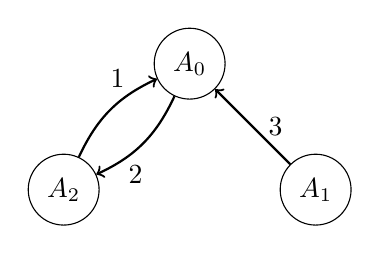
\begin{tikzpicture}[scale=0.8]
    \node[circle,draw,minimum size=0.9cm] (a) at (2,2) {$A_0$};
    \node[circle,draw,minimum size=0.9cm] (b) at (4,0) {$A_1$};
    \node[circle,draw,minimum size=0.9cm] (c) at (0,0) {$A_2$};
    \draw[->,thick] (b) -- (a) node[midway,right=2pt] {3};
    \draw[->,thick] (a) to[bend left=20] (c) node[right=8pt] {2};
    \draw[->,thick] (c) to[bend left=20] (a) node[left=8pt] {1};
\end{tikzpicture}
\end{minipage}
\begin{minipage}{0.6\textwidth}
$$
A = \begin{bmatrix}
    \infty & \infty & 2 \\
    3 & \infty & \infty \\
    1 & \infty & \infty
\end{bmatrix}
\quad \xrightarrow{\text{algorithm execution}} \quad
A^*  = \begin{bmatrix}
    \infty & \infty & 2 \\
    3 & \infty & 5 \\
    1 & \infty & 3
\end{bmatrix}
$$
\end{minipage}
\end{center}

The algorithm follows the same structure as the transitive closure computation, but with a crucial modification in the update operation. Instead of the Boolean OR operation used for reachability, each processor $p_{k,j}$ performs a distance minimization: after storing the local weight $W_{k,j}$ and receiving the flowing values $W_{i,j}$ and $W_{i,k}$, it updates $W_{i,j} \gets \min(W_{i,j}, W_{i,k} + W_{k,j})$. This operation implements the core principle of dynamic programming for shortest paths: if there exists a path from $i$ to $j$ through intermediate node $k$ with total weight $W_{i,k} + W_{k,j}$ that is shorter than the current known path weight $W_{i,j}$, then we update our estimate.

Upon completion, each matrix element $W_{i,j}$ contains the weight of the least-weight path from node $i$ to node $j$. However, knowing only the path weights is often insufficient—we typically need to reconstruct the actual sequence of nodes that constitutes the optimal path.

\textbf{Path Reconstruction.} To enable path reconstruction, we maintain an auxiliary matrix $X$ alongside the weight matrix $W$. For each pair of nodes $(i,j)$, the entry $x_{ij}$ stores the \emph{next hop} in the optimal path from $i$ to $j$. The rows of matrix $X$ flow through the systolic mesh in parallel with the corresponding rows of $W$, and the broadcast operations include both weight and next-hop information.

The initialization and update procedures for the next-hop matrix are as follows:
\begin{itemize}
    \item \textbf{Initialization:} Set $x_{ij} = j$ for all pairs $(i,j)$, indicating that the direct edge $(i,j)$ is initially considered the best path.
    \item \textbf{Update rule:} When processor $p_{k,j}$ updates the weight $W_{i,j} \gets \min(W_{i,j}, W_{i,k} + W_{k,j})$, it simultaneously updates the next-hop information:
    $$x_{ij} \gets \begin{cases}
        x_{ij} & \text{if } W_{i,j} \leq W_{i,k} + W_{k,j} \\
        x_{ik} & \text{if } W_{i,j} > W_{i,k} + W_{k,j}
    \end{cases}$$
    This ensures that $x_{ij}$ always points to the first node on the current best path from $i$ to $j$.
\end{itemize}

After the algorithm terminates, the complete least-weight path from node $i$ to node $j$ can be reconstructed by following the sequence of next-hop pointers: $i \to x_{ij} \to x_{x_{ij}j} \to x_{x_{x_{ij}j}j} \to \cdots$ until reaching the destination $j$. This reconstruction process requires at most $N-1$ steps, where $N$ is the number of nodes, since any simple path contains at most $N-1$ intermediate nodes.

So, the same network and algorithm that we used to compute the transitive closure of a graph can be used to compute shortest (least-weight) paths between all pairs of nodes. Thus, the performances of the algorithm are still those given in the previous section.


\section{Connected Components of a Graph}

Another graph problem that can take advantage of the algorithm for the transitive closure is that of finding the connected components of an undirected graph. A \bfit{connected component} is a maximal subset $S \subseteq V$ of nodes such that for every pair of nodes $i, j \in S$, there is a path from $i$ to $j$. To be maximal means that no other node $k \in V \setminus S$ in the graph is connected by a path to some node in $S$.

\vspace{-1em}

\begin{figure}[H]
\centering
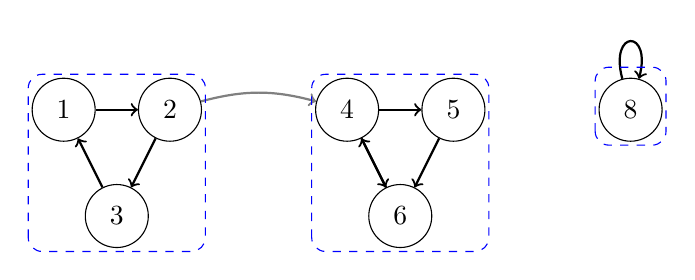
\begin{tikzpicture}[scale=0.9, node distance=1.5cm]
    % First strongly connected component
    \node[circle,draw,minimum size=0.8cm] (a1) at (0,2) {1};
    \node[circle,draw,minimum size=0.8cm] (a2) at (1.5,2) {2};
    \node[circle,draw,minimum size=0.8cm] (a3) at (0.75,0.5) {3};
    
    % Second strongly connected component
    \node[circle,draw,minimum size=0.8cm] (b1) at (4,2) {4};
    \node[circle,draw,minimum size=0.8cm] (b2) at (5.5,2) {5};
    \node[circle,draw,minimum size=0.8cm] (b3) at (4.75,0.5) {6};
    
    % Fourth component (single node with self-loop)
    \node[circle,draw,minimum size=0.8cm] (d1) at (8,2) {8};
    
    % Directed edges for first component (cycle)
    \draw[->,thick] (a1) -- (a2);
    \draw[->,thick] (a2) -- (a3);
    \draw[->,thick] (a3) -- (a1);
    
    % Directed edges for second component
    \draw[->,thick] (b1) -- (b2);
    \draw[->,thick] (b2) -- (b3);
    \draw[->,thick] (b3) -- (b1);
    \draw[->,thick] (b1) -- (b3);
    
    % Self-loop for fourth component
    \draw[->,thick] (d1) to[loop above] (d1);
    
    % Inter-component edges (these don't affect strong connectivity)
    \draw[->,thick,gray] (a2) to[bend left=15] (b1);
    
    % Dashed boundaries around strongly connected components
    \draw[dashed,blue,rounded corners=5pt] (-0.5,0) rectangle (2,2.5);
    \draw[dashed,blue,rounded corners=5pt] (3.5,0) rectangle (6,2.5);
    \draw[dashed,blue,rounded corners=5pt] (7.5,1.5) rectangle (8.5,2.6);
\end{tikzpicture}
\caption{A graph with three connected components.}
\label{fig:connected-components}
\end{figure}

\vspace{-1.5em}

First, we compute the transitive closure $A^*$ of the adjacency matrix. Then, $A^*_{ij} = 1$ if and only if nodes $i$ and $j$ are in the same connected component. So, it is enough to associate each node $i \in V$ with the index $k = \min \{j \mid A^*_{ij} = 1\}$, that is, the leftmost 1 in the row $i$ of the matrix. Nodes associated with the same index $k$ form a connected component, one for each different $k$.

Again, performances are similar to those of the transitive closure algorithm since the added steps, which take place after computing the transitive closure, can still be performed on the same mesh network in linear time (in parallel). However, note that the speedup and efficiency are not as good, because it exists a sequential algorithm which is able to compute the connected components in just $O(|E|)$ steps.

\section{Matrix Multiplication}

Matrix multiplication is a classical problem for which a number of algorithms have been proposed, both sequential and parallel. For simplicity we will restrict to the product of square matrices. Given two square matrices $A$ and $B$ of size $N \times N$, we want to compute their product $C = A \cdot B$, where each element is defined by $C_{i,j} = \sum_{k=0}^{N-1} A_{i,k} B_{k,j}$, for every $0 \leq i,j \leq N-1$. Moreover, we want to do this on a torus of size $N \times N$, so with $P = N^2$ processors with each constant memory $M = 3$.

Since each processor $p_{i,j}$ of the network has only constant memory $M = 3$, the two input matrices must be both distributed (one element per processing unit). So, initially processor $p_{i,j}$ will contain elements $A_{i,j}$ and $B_{i,j}$ of the input matrices. The third memory cell will instead be used to store the corresponding element $C_{i,j}$ of the product. Initially, every $C_{i,j} = 0$. Observe that some processors cannot use their initial input values right away. For instance, processor $p_{0,1}$ cannot immediately compute any component of the sum $C_{0,1} = A_{0,0} B_{0,1} + A_{0,1} B_{1,1} + \cdots + A_{0,N-1} B_{N-1,1}$, since its input values are $A_{0,1}$ and $B_{0,1}$. Therefore, to avoid idle waiting, the algorithm must first move the data to a configuration where each processing unit contains a pair of input values that can immediately use for computing one addend of the corresponding element of $C$. To understand what such a configuration could be, we first give an example. Suppose $N = 3$.

$$
\begin{array}{l}
C_{0,0} = \color{blue} A_{0,0} B_{0,0} \color{black} + A_{0,1} B_{1,0} + A_{0,2} B_{2,0} \\
C_{0,1} = A_{0,0} B_{0,1} + \color{blue} A_{0,1} B_{1,1} \color{black} + A_{0,2} B_{2,1} \\
C_{0,2} = A_{0,0} B_{0,2} + A_{0,1} B_{1,2} + \color{blue} A_{0,2} B_{2,2} \color{black} \\
\end{array}
\quad
\begin{array}{l}
C_{1,0} = A_{1,0} B_{0,0} + A_{1,1} B_{1,0} + \color{blue} A_{1,2} B_{2,0} \color{black} \\
C_{1,1} = \color{blue} A_{1,0} B_{0,1} \color{black} + A_{1,1} B_{1,1} + A_{1,2} B_{2,1} \\
C_{1,2} = A_{1,0} B_{0,2} + \color{blue} A_{1,1} B_{1,2} \color{black} + A_{1,2} B_{2,2} \\
\end{array}
$$
$$
\begin{array}{l}
C_{2,0} = A_{2,0} B_{0,0} \color{blue} + A_{2,1} B_{1,0} \color{black} + A_{2,2} B_{2,0} \\
C_{2,1} = A_{2,0} B_{0,1} + A_{2,1} B_{1,1} \color{blue} + A_{2,2} B_{2,1} \color{black} \\
C_{2,2} = \color {blue}A_{2,0} B_{0,2} \color{black} + A_{2,1} B_{1,2} + A_{2,2} B_{2,2} \\
\end{array}
$$
$$
\color{blue} \blacksquare \color{black} \text{ Possible elements that can be computed immediately after initial data placement}
$$

Now, for each $C_{i,j}$, we need to find a pair of values $A_{i,k}$ and $B_{k,j}$ such that they will not be chosen for any other $C_{i',j'}$. This is due to the fact that all inputs must still be uniquely distributed, a different pair to each processing unit. There are many configurations that satisfy such conditions, even just by symmetry.

\vspace{-1em}

\begin{figure}[H]
    \centering
    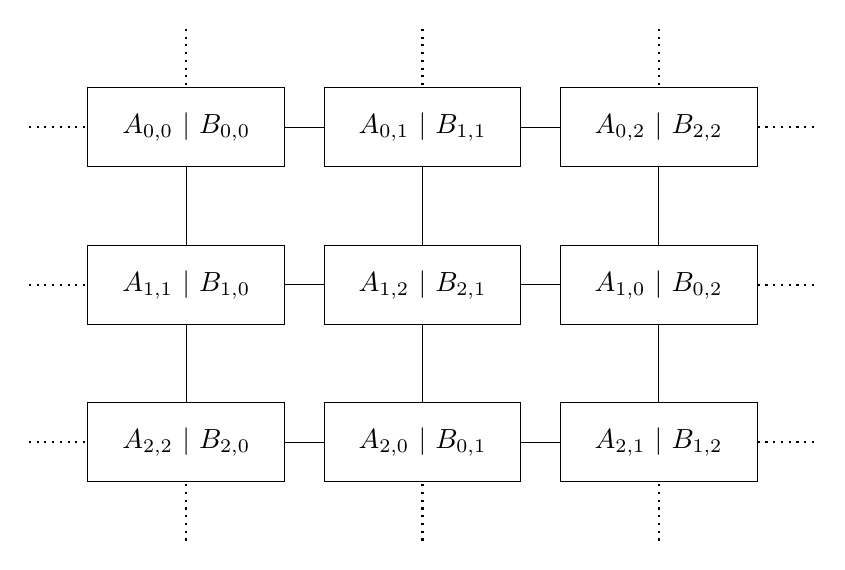
\begin{tikzpicture}[scale=1, every node/.style={draw, minimum width=2.5cm, minimum height=1cm, font=\normalsize}]
        % Nodes
        \node (a00) at (0,2) {$A_{0,0}\ |\ B_{0,0}$};
        \node (a01) at (3,2) {$A_{0,1}\ |\ B_{1,1}$};
        \node (a02) at (6,2) {$A_{0,2}\ |\ B_{2,2}$};
        
        \node (a10) at (0,0) {$A_{1,1}\ |\ B_{1,0}$};
        \node (a11) at (3,0) {$A_{1,2}\ |\ B_{2,1}$};
        \node (a12) at (6,0) {$A_{1,0}\ |\ B_{0,2}$};
        
        \node (a20) at (0,-2) {$A_{2,2}\ |\ B_{2,0}$};
        \node (a21) at (3,-2) {$A_{2,0}\ |\ B_{0,1}$};
        \node (a22) at (6,-2) {$A_{2,1}\ |\ B_{1,2}$};
        
        % Horizontal lines
        \draw (a00) -- (a01);
        \draw (a01) -- (a02);
        \draw (a10) -- (a11);
        \draw (a11) -- (a12);
        \draw (a20) -- (a21);
        \draw (a21) -- (a22);
        
        % Vertical lines
        \draw (a00) -- (a10);
        \draw (a10) -- (a20);
        \draw (a01) -- (a11);
        \draw (a11) -- (a21);
        \draw (a02) -- (a12);
        \draw (a12) -- (a22);
        
        % Dotted lines for torus wraparound (horizontal)
        \draw[dotted, thick] (-2,2) -- (a00);
        \draw[dotted, thick] (a02) -- (8,2);
        \draw[dotted, thick] (-2,0) -- (a10);
        \draw[dotted, thick] (a12) -- (8,0);
        \draw[dotted, thick] (-2,-2) -- (a20);
        \draw[dotted, thick] (a22) -- (8,-2);
        
        % Dotted lines for torus wraparound (vertical)
        \draw[dotted, thick] (0,3.25) -- (a00);
        \draw[dotted, thick] (3,3.25) -- (a01);
        \draw[dotted, thick] (6,3.25) -- (a02);
        \draw[dotted, thick] (0,-3.25) -- (a20);
        \draw[dotted, thick] (3,-3.25) -- (a21);
        \draw[dotted, thick] (6,-3.25) -- (a22);
    \end{tikzpicture}
    \caption{A distribution of the input allowing each processor to perform some computation.}
    \label{fig:matrix-multiplication}
\end{figure}

\vspace{-1.5em}

Let us analyze the configuration shown in \cref{fig:matrix-multiplication}. Initially, each processor $p_{i,j}$ holds elements $A_{i,j}$ and $B_{i,j}$. The data movement pattern reveals that each row $i$ of matrix $A$ undergoes a leftward rotation by $i$ positions, while each column $j$ of matrix $B$ rotates upward by $j$ positions. This pattern generalizes to any dimension $N$: after the rotations, processor $p_{i,j}$ contains elements $A_{i,k}$ and $B_{k,j}$, where $k = i+j \mod N$. The initial data movement phase requires $N - 1$ steps to achieve this configuration, since the last row of $A$ and last column of $B$ must move $N - 1$ positions. We assume this initial configuration is not provided, making this phase necessary.

The computation phase alternates between arithmetic operations and communication steps. In each step, processor $p_{i,j}$:
\begin{enumerate}
    \item Updates its partial result: $C_{i,j} = C_{i,j} + A_{i,k} \cdot B_{k,j}$
    \item Forwards $A_{i,k}$ to its left neighbor and $B_{k,j}$ upward
    \item Receives new values $A_{i,k'}$ and $B_{k',j}$ from right and below, where $k' = k+1 \mod N$
\end{enumerate}
This creates a continuous rotation pattern: rows of $A$ shift leftward while columns of $B$ shift upward. After $N$ such steps, each processor has processed all required value pairs for its final computation. The total execution time is $2N - 1$ steps ($N - 1$ for initial configuration plus $N$ for computation), after which the torus contains the complete product matrix $C$.

The algorithm extends naturally to cases where $P < N^2$ processors are available, forming a $\sqrt{P} \times \sqrt{P}$ torus (assuming $N$ is a multiple of $\sqrt{P}$). Here, we employ block distribution: each processor $p_{i,j}$ manages $n \times n$ blocks $A(i,j)$ and $B(i,j)$, where $n = N/\sqrt{P}$. The block $A(i,j)$ has the following structure:
$$
A(i,j) = 
\begin{bmatrix}
A_{in,\,jn} & A_{in,\,jn+1} & \cdots & A_{in,\,(j+1)n-1} \\
A_{in+1,\,jn} & A_{in+1,\,jn+1} & \cdots & \vdots \\
\vdots & \ddots & \ddots & \vdots \\
A_{(i+1)n-1,\,jn} & \cdots & \cdots & A_{(i+1)n-1,\,(j+1)n-1}
\end{bmatrix}
$$

The block structure for $B(i,j)$ follows the same pattern as $A(i,j)$. In this block-based approach, each processor $p_{i,j}$ computes its corresponding block $C(i,j)$ of the product matrix $C$. This requires increased memory per processor: $M = 3N^2/P$ elements, which grows with the problem size. The algorithm maintains the same two-phase structure as before, but operates on blocks rather than individual elements.

The block-based algorithm proceeds as follows:
\begin{enumerate}
    \item \textbf{Initial Configuration Phase:} Each row $i$ rotates its blocks $A(i,\,\_)$ leftward by $i$ positions, while each column $j$ rotates its blocks $B(\_,\,j)$ upward by $j$ positions.
    \item \textbf{Computation Phase:} In each step, processor $p_{i,j}$:
    \begin{itemize}
        \item Updates its block: $C(i,j) = C(i,j) + A(i,k) \cdot B(k,j)$
        \item Forwards blocks $A(i,k)$ leftward and $B(k,j)$ upward
    \end{itemize}
\end{enumerate}

Note that now the steps are not constant any more, not even the communications, since they involve blocks of $N^2/P$ elements. Furthermore, the arithmetical operations require to compute a matrix product, since the blocks $A(i,k)$ and $B(k,j)$ are actually matrices. On the other hand, the two phases take just $\sqrt{P} - 1$ and $\sqrt{P}$ steps, respectively.

\subsection*{Performances}

\begin{itemize}
    \item The \textbf{parallel execution time} is $T_{N^2}(N) = \Theta(N)$ since the procedure takes $2N - 1$ constant steps, then the work is $W = \Theta(N^3)$.
    \item The \textbf{speedup} is $S = O(N^{2.37})/\Theta(N) = O(N^{1.37})$ w.r.t.\ the fastest sequential algorithm (although, as already mentioned, such an algorithm is actually impractical due to the huge constants), then the \textbf{efficiency} is $\varepsilon = O(N^{1.37}/N^2) = O(1/N^{0.63})$.
\end{itemize}

\begin{tipsblock}[Matrix multiplication]
    Element $A_{i,j}$ stays in row $i$ but moves leftward by $i$ positions, while element $B_{j,i}$ stays in column $i$ but moves upward by $j$ positions. This means that their new index will be:
    $$
    A_{i,j} \to A_{i, (j-i)} \quad \text{and} \quad B_{j,i} \to B_{(j-i), i}
    $$
    Thus, in processor $p_{i,j}$ we will have the elements:
    $$
    A_{i,(j+i)} \quad \text{and} \quad B_{(i+j), j}
    $$
    where all indices are taken modulo $N$.
\end{tipsblock}